\documentclass[tikz]{standalone}
\usepackage{pgfplots}
\pgfplotsset{width=14.cm, height=9cm, compat=1.18}
\usepackage{tikz}
\usepackage{amsmath}

\definecolor{darkgray176}{RGB}{176,176,176}
\definecolor{green01780}{RGB}{0,178,0}

\begin{document}
	
	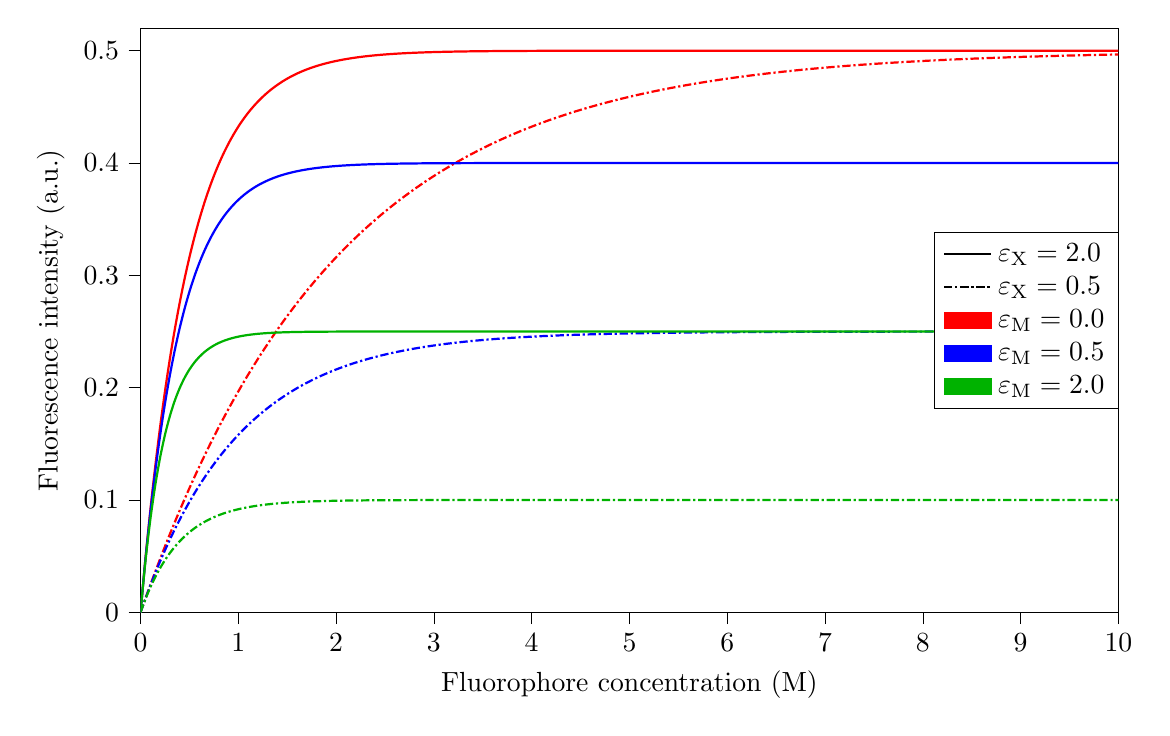
\begin{tikzpicture}
		\begin{axis}[
			tick align=outside,
			tick pos=left,
			x grid style={black},
			xlabel={Fluorophore concentration (M)},
			xmin=0, xmax=10,
			xtick style={color=black},
			y grid style={black},
			ylabel={Fluorescence intensity (a.u.)},
			ymin=0, ymax=0.52,
			ytick style={color=black},
			legend style={at={(1,0.5)},anchor=east, xshift=+0.2pt, yshift=+0.pt,
			%legend image post style={line width=2pt},
			},
			legend cell align=left,
			]
			% Legend dummy plots
			\addplot[draw=black, thick] (1,1);
			\addplot[draw=black, thick, densely dashdotted] (1,1);
			\addplot[draw=red, fill=red, area legend] (1,1);
			\addplot[draw=blue, fill=blue, area legend] (1,1);
			\addplot[draw=green01780, fill=green01780, area legend] (1,1);
			% Curves
			\addplot[domain = 0:10,	samples = 200, smooth,
			thick, red,] {1/2*2/(2+0)*(1-exp(-x*(2+0)))};
			\addplot[domain = 0:10,	samples = 200, smooth,
			thick, red, densely dashdotted] {1/2*0.5/(0.5+0)*(1-exp(-x*(0.5+0)))};
			\addplot[domain = 0:10,	samples = 200, smooth,
			thick, blue,] {1/2*2/(2+0.5)*(1-exp(-x*(2+0.5)))};
			\addplot[domain = 0:10,	samples = 200, smooth,
			thick, blue, densely dashdotted] {1/2*0.5/(0.5+0.5)*(1-exp(-x*(0.5+0.5)))};
			\addplot[domain = 0:10,	samples = 200, smooth,
			thick, green01780,] {1/2*2/(2+2)*(1-exp(-x*(2+2)))};
			\addplot[domain = 0:10,	samples = 200, smooth,
			thick, green01780, densely dashdotted] {1/2*0.5/(0.5+2)*(1-exp(-x*(0.5+2)))};
			\legend{
				$\varepsilon_\text{X}=2.0$,
				$\varepsilon_\text{X}=0.5$,
				$\varepsilon_\text{M}=0.0$,
				$\varepsilon_\text{M}=0.5$,
				$\varepsilon_\text{M}=2.0$}
		\end{axis}
	\end{tikzpicture}
	
\end{document}